\paragraph{RLPBWT.}
In merito alle varianti della $\RLPBWT$, sono state testate le otto
strutture dati composte discusse nel capitolo \ref{metchap}:
\begin{enumerate}
  \item la struttura dati composta \texttt{MAP-INT + LCP} e la struttura dati
  composta \texttt{MAP-BV + LCP}. Si ricorda che tali soluzioni non supportano
  il riconoscimento delle righe del pannello per cui si ha uno $\SMEM$ ma
  solo la cardinalità dell'insieme di tali righe
  \item le strutture dati composte basate sull'uso delle threshold per
  il calcolo dell'array delle matching statistics, 
  ovvero: \texttt{MAP-INT + THR-INT + RA-BV + PERM + PHI},  \texttt{MAP-INT +
    THR-INT + RA-SLP + PERM + PHI}, \texttt{MAP-BV + THR-BV + RA-BV + PERM +
    PHI} e \texttt{MAP-BV + THR-BV + RA-SLP + PERM + PHI} 
  \item le strutture dati composte basate sull'uso delle $\LCE$ query
  per
  il calcolo dell'array delle matching statistics,
  ovvero: \texttt{MAP-INT + LCE + PERM + PHI} e \texttt{MAP-BV + LCE + PERM +
    PHI}  
\end{enumerate}
L'implementazione è stata fatta in linguaggio \Cplusplus, usando le già citate
librerie esterne:
\begin{itemize}
  \item SDSL per intvector compressi,
  bitvector, bitvector sparsi, serializzazione e varie utility
  per il calcolo della memoria delle strutture dati
  \item BigRePair e ShapedSlp per la costruzione e l'uso degli $\SLP$ 
\end{itemize}
L'implementazione delle strutture composte per la
$\RLPBWT$ supporta lo studio parallelo di più query tramite
openMP \cite{openmp}. Al fine di un più 
corretto confronto con l'implementazione della $\PBWT$,
l'intera sperimentazione è stata
svolta sfruttando un solo thread per volta, tramite la variabile
d'ambiente \texttt{OMP\_NUM\_THREADS=1}.
\paragraph{PBWT.}
Al fine di validare più correttamente i confronti tra le varie strutture dati
per la $\RLPBWT$ e la $\PBWT$ di Durbin, si è scelto di utilizzare
l'implementazione originale di
quest'ultima\footnote{\url{https://github.com/richarddurbin/pbwt}}. Tale
implementazione è scritta in 
linguaggio C. L'implementazione
fornisce tre algoritmi per il calcolo degli $\SMEM$, avendo $N$ siti, $M$ sample
e $Q$ query, per i quali si riportano le complessità asintotiche specificate
nei commenti del codice: 
\begin{enumerate}
  \item \texttt{matchNaive}, ovvero un'implementazione na\"{i}ve del calcolo
  degli $\SMEM$ che non sfrutta la $\PBWT$. Questo algoritmo non è
  utilizzabile in casi reali. La complessità in tempo di tale 
  soluzione è stimata essere $\mathcal{O}(NMQ)$ mentre quella in spazio è
  $\mathcal{O}(NM)$
  \item \texttt{matchIndexed}, ovvero l'algoritmo 5 del paper originale
  \cite{pbwt}. La complessità in tempo di tale 
  soluzione è stimata essere $\mathcal{O}(NQ)$, dopo una fase di preprocessing
  con complessità $\mathcal{O}(NM)$. La complessità in spazio è stimata essere
  $\mathcal{O}(NM)$, ricordando che, in pratica, essa corrisponda a $13NM$
  byte in memoria
  \item \texttt{matchDynamic}, ovvero un algoritmo non approfondito nel paper ma
  solo citato nei risultati sotto il nome di ``batch''. Pur mancando una
  descrizione approfondita dell'algoritmo, si è dedotto che il suo funzionamento
  si basi sul creare una trasformata $\PBWT$ anche delle query, viste 
  sotto forma di pannello, e applicare l'algoritmo per il calcolo degli $\SMEM$
  interni alla $\PBWT$ stessa. Inoltre, il calcolo dei vari indici viene
  fatto di colonna in colonna, dovendo fare, a differenza dell'algoritmo
  \texttt{matchIndexed} e degli algoritmi per la $\RLPBWT$, una sola scansione
  della struttura dati per tutte le query. La complessità in tempo di tale 
  soluzione è stimata essere $\mathcal{O}(N(M+Q))$ mentre quella in spazio è
  $\mathcal{O}(N+M)$. 
\end{enumerate}
Si intuisce fin da subito come l'ultima soluzione, non approfondita nel paper di
riferimento e della quale si è avuto riconoscimento solo in fase di
sperimentazione, risulti essere la migliore a disposizione. Si hanno solo due
piccole limitazioni. La prima è dovuta al fatto che, dovendo di fatto computare
la trasformata anche per il pannello di query ed essendo l'algoritmo studiato
per lavorare sulla trasformata stessa, i tempi di calcolo per poche query sono
alti rispetto all'algoritmo \texttt{matchIndexed} e rispetto alle varie
soluzioni per la $\RLPBWT$. Il secondo limite è che i risultati non sono
ordinati. Tutti gli altri algoritmi presentano i risultati query per query, in
ordine, mentre l'algoritmo \texttt{matchDynamic}, studiando la trasformata anche
delle query,
presenta tutti i risultati permutati secondo la stessa. Si rileva, in ogni caso,
come tali limiti possano essere per lo più trascurati, nonostante il problema su
cui si concentrano gli studi di questa tesi fosse la ricerca degli $\SMEM$ tra
una 
singola query e un pannello di aplotipi.
\section{Pannelli del 1000 Genome Project}
Come anticipato, al fine di valorizzare i risultati teorici ottenuti in
questo progetto, si 
è deciso di procedere con lo studio di dati reali, relativi alla phase
  3 del 1000 Genome Project
\footnote{\url{https://ftp.1000genomes.ebi.ac.uk/vol1/ftp/release/20130502/}}
\cite{1kgp}.\\ 
Tali pannelli, disponibili in formato VCF (Variant Call Format) \cite{vcf},
presentano un numero 
costante di sample, ovvero 5.008, mentre a variare è il numero di siti. Essendo
dati reali, si ha anche la presenza di siti multiallelici. Si è quindi proceduto
alla selezione dei soli siti biallelici, ottenendo pannelli costruiti su
un alfabeto binario $\Sigma=\{0,1\}$, tramite l'uso di \textit{bcftools}
\cite{bcftools}, tramite il comando \texttt{bcftools view -m2 -M2
  -v snps}.\\
La prima selezione dei pannelli è stata dettata dalla volontà di studiare, per
praticità, pannelli non troppo estesi, ad eccezione di uno molto grande. Si
sono, 
quindi, scelti i pannelli relativi ai cromosomi 22 (\texttt{chr22}), 20
(\texttt{chr20}), 18 (\texttt{chr18}), 16 (\texttt{chr16}) e 1 (\texttt{chr1}).
Si noti che  
l'ordine è dato dal numero crescente di siti. La scelta di includere il
cromosoma 1 è dettata dal fatto che risulta essere il più grande cromosoma
umano, implicando che anche il relativo pannello delle variazioni geniche
sia tra quelli col maggior numero di siti.\\
Trattandosi di pannelli reali, è risultata interessante una preliminare
indagine esplorativa sulla natura di tali pannelli in termini di
sparsità degli alleli e di conseguente attesa numerosità delle run. Si è
quindi calcolato, per i cinque pannelli, il numero di simboli $\sigma=0$ e
$\sigma=1$, notando come il numero di simboli $\sigma=1$ fosse molto ridotto
rispetto al totale, essendo il $\sim 0.03\%$ del totale dei simboli in tutti e
cinque i casi. Una tale
sparsità del dato ha diretta conseguenza sul numero di run di ogni
colonna. Infatti, avendo 
pochi simboli $\sigma=1$ in ogni colonna, simboli che possono anche
essere nella medesima run dopo la permutazione data dalla
$\PBWT$, si producono, nel complesso, poche run. Si ricordi, inoltre, che tale
permutazione, come la 
$\BWT$, è studiata per essere 
maggiormente efficiente nel caso del dato biologico, comportando un'alta
probabilità di produrre run del medesimo carattere. In tabella \ref{tab:panel},
quindi, si riportano il numero di siti di ogni cromosoma, il 
numero medio di run per colonna, il numero 
massimo di run in una colonna e il totale delle run. Si segnala, inoltre,
come la
mediana del numero di run per colonna abbia valore 3 per tutti e tre i pannelli.
I valori quantitativi sono 
stati calcolati a partire dai pannelli con un numero di sample pari a 4.908 in
quanto, si anticipa, 100 righe sono state utilizzate come query nelle successive
fasi della sperimentazione.
\begin{table}
  \centering
  \caption{Informazioni quantitative relative ai cinque pannelli in analisi.}
  \label{tab:panel}
  \begin{tabular}{c||c|c|c|c}
    \textbf{Chr} & \textbf{\#Siti} & \textbf{\#Run totale}
    & \textbf{Max run} & \textbf{Media run} \\ 
    \hline
    \texttt{chr22} & 1.055.454 & 14.772.105 & 2.450 & 14\\
    \texttt{chr20} & 1.739.315 & 19.966.504 & 2.176 & 11\\
    \texttt{chr18} & 2.171.378 & 24.288.263 & 2.365 & 11\\
    \texttt{chr16} & 2.596.072 & 31.187.856 & 2.330 & 12\\
    \texttt{chr1} & 6.196.151 & 69.671.952 & 2.721 & 11\\
  \end{tabular}
\end{table}
Si conferma il risultato atteso, in merito alla sparsità del dato e al
conseguente basso numero medio di run per colonna, risultato che è a favore, in
termini di 
complessità in spazio, della $\RLPBWT$, in quanto tutte le componenti sono
proporzionali al numero di run (ad eccezione della componente \texttt{RLCP}). In
figura 
\ref{fig:boxplot} si riportano i risultati statistici, sotto forma di
boxplot, relativi alla distribuzione delle run nei cinque pannelli
studiati. Il forte numero di outlier è dovuto al fatto che media e sopratutto
mediana del numero di run per colonna risultino essere molto piccoli rispetto al
numero massimo di run riscontrabili in una colonna.
\begin{figure}
  \centering
  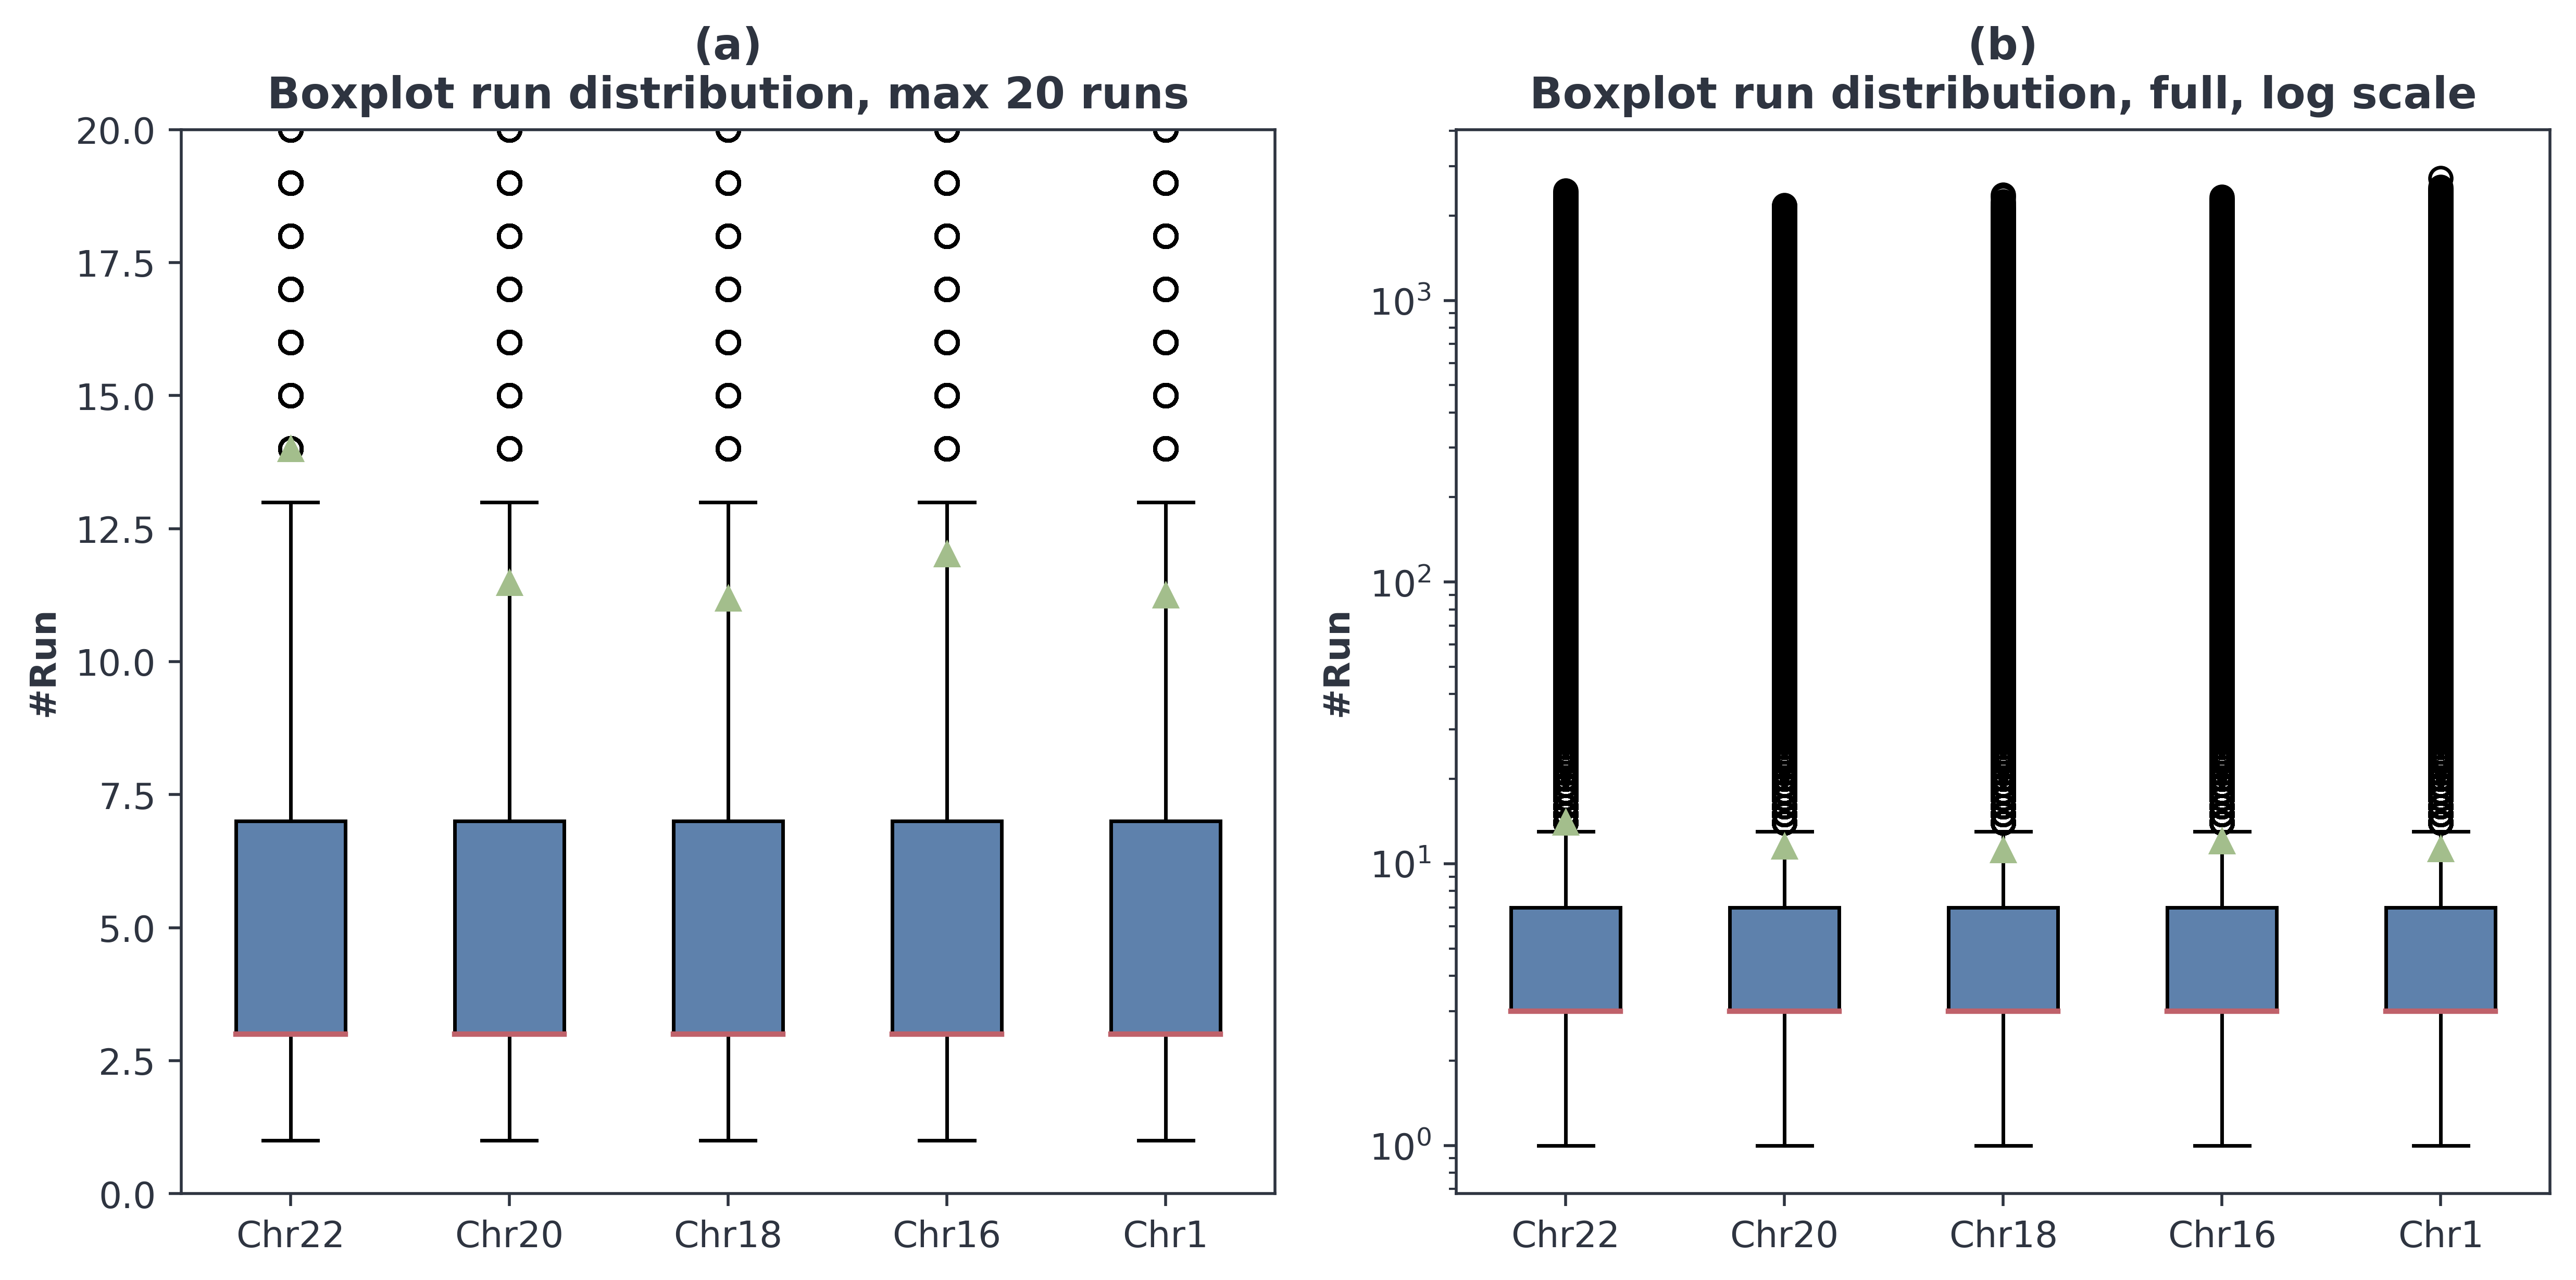
\includegraphics[width = \linewidth]{img/boxplotbi.png}
  \caption{Boxplot della distribuzione delle run per i pannelli dei cinque
    cromosomo studiati. Il grafico (a) presenta uno zoom che esclude la maggior
    parte degli outlier mentre il grafico (b) presenta, in scala logaritmica, il
    boxplot completo con tutti gli outlier.}
  \label{fig:boxplot}
\end{figure}
\subsection{Riproducibilità degli esperimenti}
Al fine di rendere riproducibili gli esperimenti, si è costruita una pipeline
per l'esecuzione dei vari algoritmi e l'estrazione dei dati quantitativi
relativi alle performance.\\
L'intera pipeline è stata gestita tramite Snakemake \cite{snakemake}
(un workflow management system), che è uno strumento molto usato in
bioinformatica per creare analisi dati scalabili e riproducibili. Nel
dettaglio la pipeline comprende, come visualizzabile in figura \ref{fig:snake},
avendo in input una lista di pannelli con associato il numero di query:
\begin{itemize}
  \item lo scaricamento dei tool e delle dipendenze per la $\PBWT$ di
  Durbin e la $\RLPBWT$ proposta in questa tesi
  \item la produzione dell'input per la $\PBWT$ e della $\RLPBWT$ per
  la quantità di query richiesta
  \item la produzione delle strutture dati
  \item l'esecuzione degli algoritmi per il calcolo degli $\SMEM$
  % \item produzione di vari grafici relativi sia ai tempi di esecuzione che alla
  % memoria richiesta
\end{itemize}
Al fine di ottenere risultati non banali, si è deciso di estrarre dai pannelli
un numero di
righe pari al numero di 
query richieste, righe che, a loro volta, andranno a formare il pannello di
query.\\
\dc{la pic va aggiornata e va aggiunto link github dopo sistemazione pipeline}
\begin{figure}
  \centering
  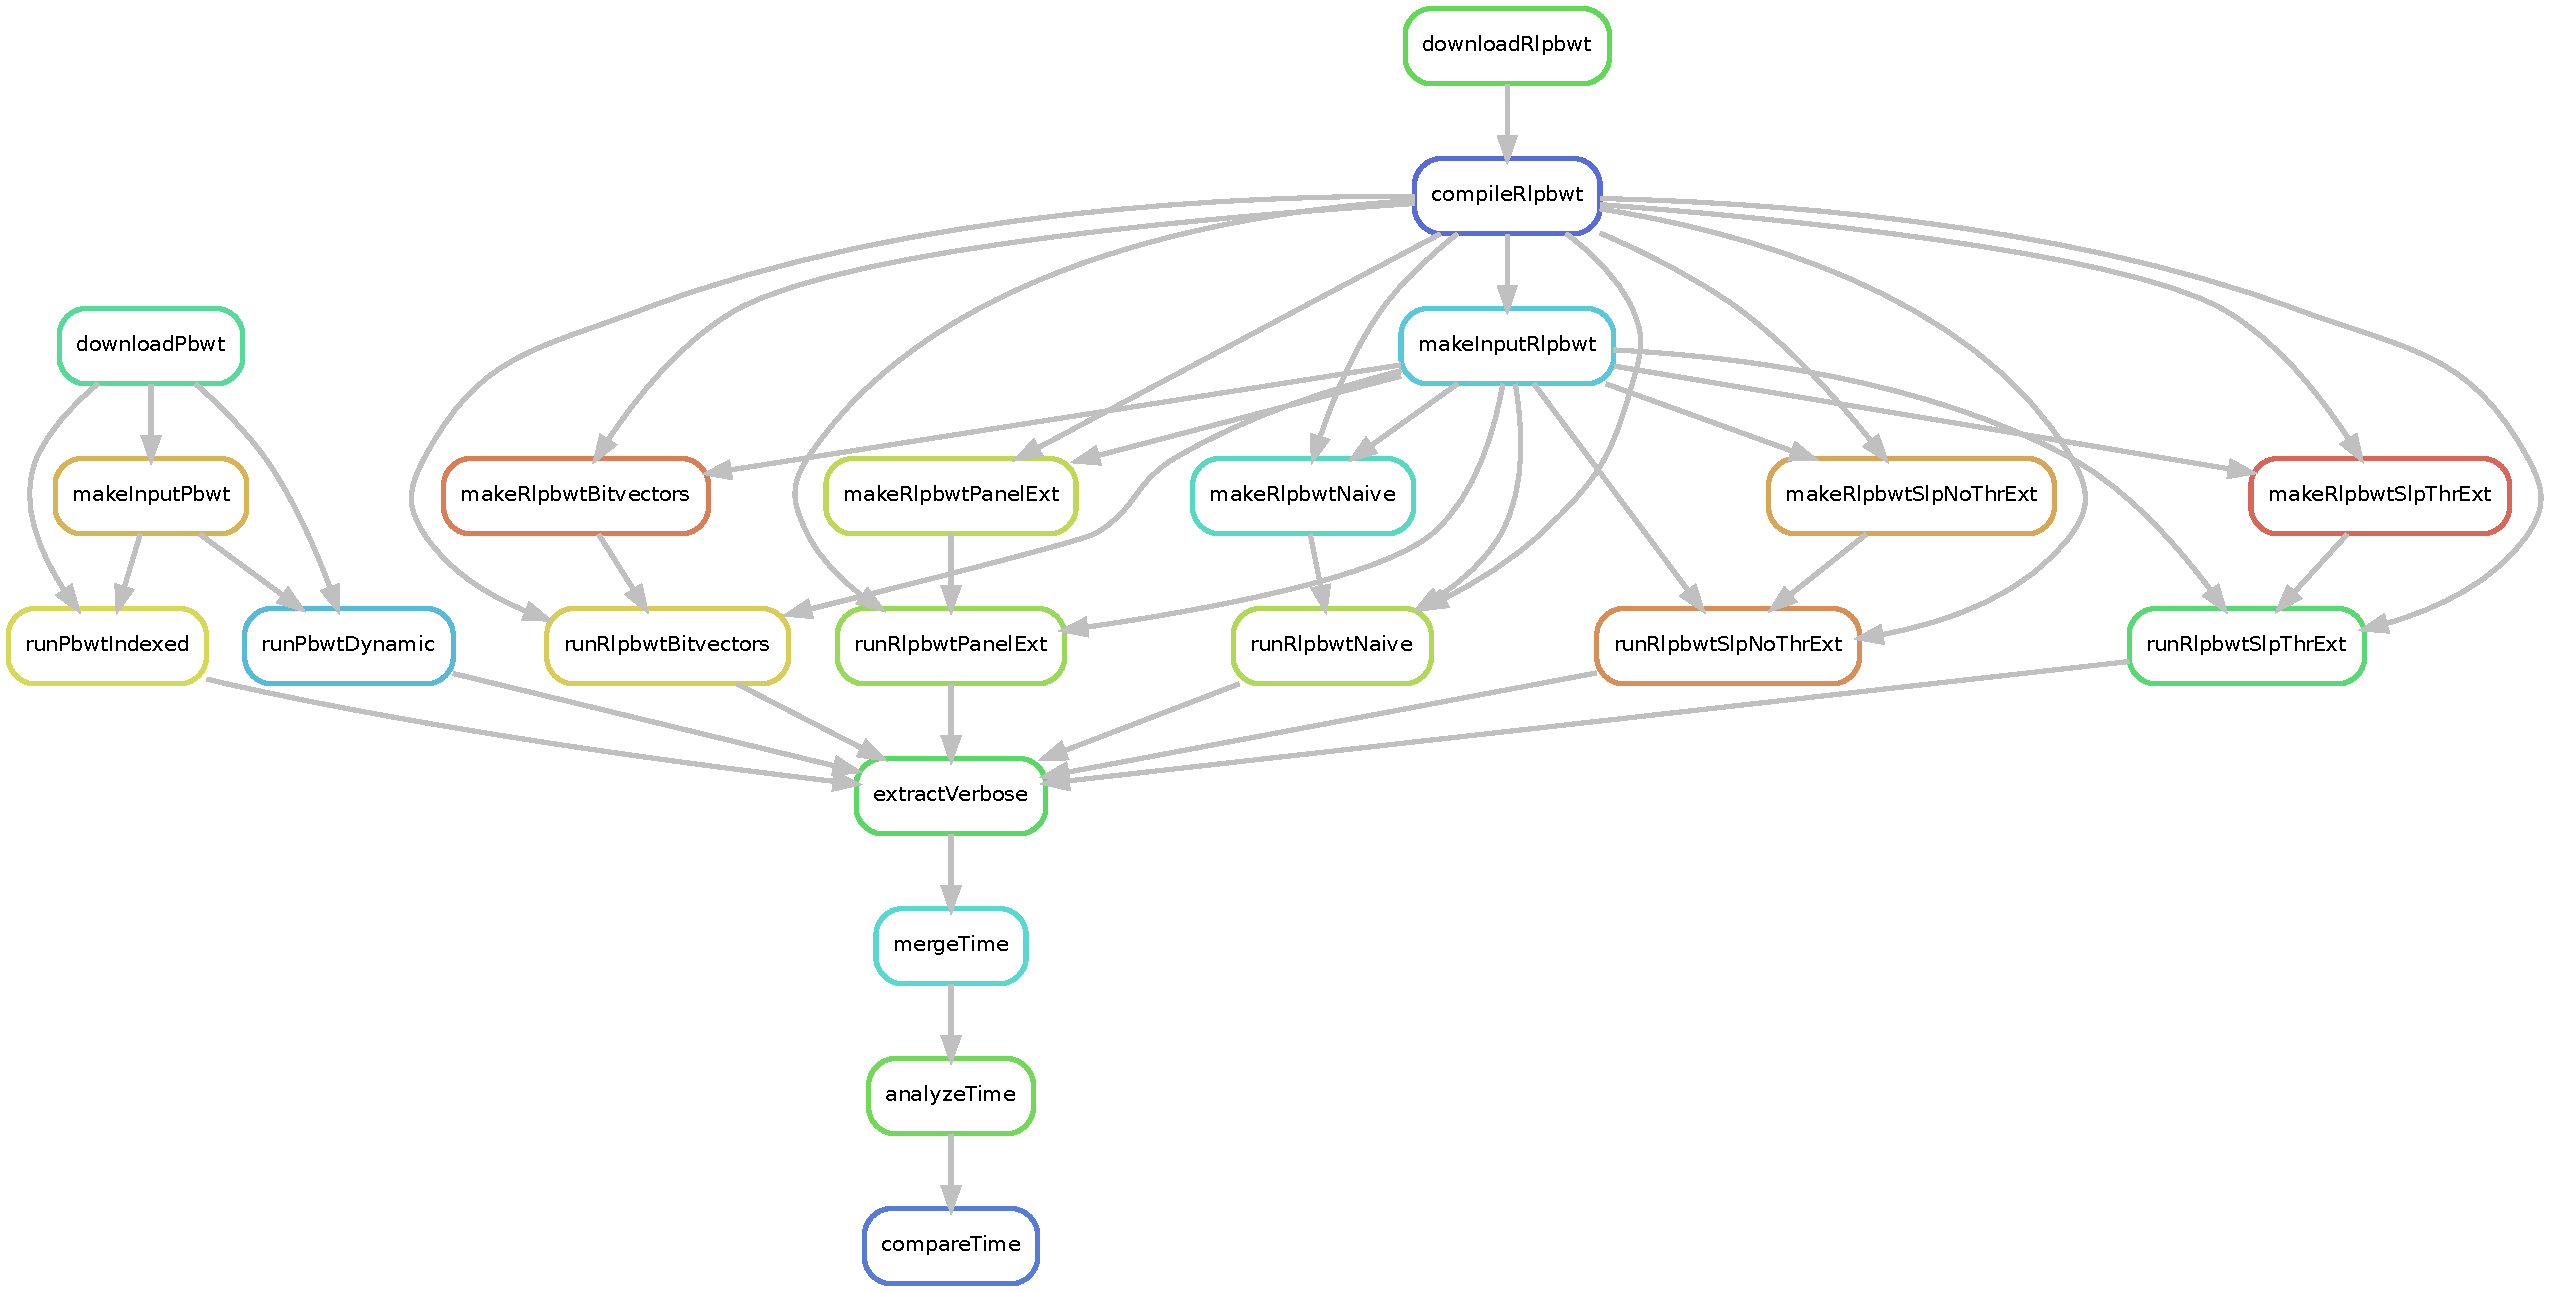
\includegraphics[width=\textwidth]{img/rules.pdf}
  \caption{Regole usate in Snakemake per la sperimentazione.}
  \label{fig:snake}
\end{figure}
\newline
\textit{La sperimentazione è stata effettuata su una macchina con processore
  Intel Xeon E5-2640 V4 ($2,40$GHz), $756$GB di RAM, $768$GB di swap e
  sistema operativo Ubuntu 20.04.4 LTS. Tale macchina è stata gentilmente messa
  a disposizione dalla \emph{University of Florida}.}